%------------------------------------------------------------------------------
% Template file for the submission of papers to IUCr journals in LaTeX2e
% using the iucr document class
% Copyright 1999-2013 International Union of Crystallography
% Version 1.6 (28 March 2013)
%------------------------------------------------------------------------------
%
%
\documentclass{iucr}
% \documentclass[preprint]{iucr}              % DO NOT DELETE THIS LINE
\usepackage{bm}
% \usepackage{graphicx}
% \usepackage{tabularx}
% \usepackage{subfigure}
% \usepackage{afterpage}
% \usepackage{sansmath}
\usepackage{mathtools}
% \usepackage{parskip}
% \usepackage{tikz}
% \usepackage{tikzorbital}
% \usepackage{setspace}
% \usepackage{xcolor}
\usepackage{amssymb}
% \usepackage{bm}
\usepackage{amsmath}
% \usepackage{fancyhdr}
% \usepackage{rotating}
\usepackage{siunitx}
\usepackage{booktabs}
\usepackage{url}
\usepackage{color}
%\usepackage{cprotect}
\usepackage{textgreek}
\usepackage[normalem]{ulem}
\usepackage{makecell}
\usepackage{cancel}
\usepackage{empheq}
\usepackage[usenames,dvipsnames]{xcolor}



% %%%%%%%%%%%%%%%%
% \usepackage[utf8]{inputenc}
% \usepackage[]{graphicx}
% \usepackage{rotating}
% \usepackage{hyperref}
% \usepackage{listings}

% \lstset{language=Fortran,
%         keywordstyle=\color{blue}\textbf,
% 	commentstyle=\color[rgb]{0.133,0.545,0.133},
% 	stringstyle=\color[rgb]{0.627,0.126,0.941},
% 	breaklines=true,
% 	showstringspaces=false,
% 	frame=trBL, basicstyle=\scriptsize %\small %\tiny %\footnotesize
%        }
% %%%%%%%%%%%%%%%%







\definecolor{darkblue}{rgb}{0.0, 0.0, 0.55}
\definecolor{cyan(process)}{rgb}{0.0, 0.72, 0.92}

\newcommand{\todo}[1]{{\color{red}[TODO: "#1'']}}
\newcommand{\inblue}[1]{{\color{blue}#1}}
\newcommand{\cyan}[1]{{\color{cyan(process)}#1}}
\newcommand{\inred}[1]{{\color{red}#1}}
\newcommand{\ingreen}[1]{{\color{green}#1}}



%%%%%%%%%%%%%%%%%%% subsubsubsection (see: https://tex.stackexchange.com/questions/60209/how-to-add-an-extra-level-of-sections-with-headings-below-subsubsection )
% \setcounter{secnumdepth}{5}
% \setcounter{tocdepth}{5}

% \makeatletter
% \newcommand\subsubsubsection{\@startsection{paragraph}{4}{\z@}{-2.5ex\@plus -1ex \@minus -.25ex}{1.25ex \@plus .25ex}{\normalfont\normalsize\bfseries}}
% \newcommand\subsubsubsubsection{\@startsection{subparagraph}{5}{\z@}{-2.5ex\@plus -1ex \@minus -.25ex}{1.25ex \@plus .25ex}{\normalfont\normalsize\bfseries}}
% \makeatother
%%%%%%%%%%%%%%%%%%%
\makeatletter
\@ifclasswith{iucr}{preprint}{
\newcommand{\whencolumns}[2]{#1}
}{
\newcommand{\whencolumns}[2]{#2}
}
\makeatother

     %-------------------------------------------------------------------------
     % Infobrmation about journal to which submitted
     %-------------------------------------------------------------------------
     \journalcode{X}              % Indicate the journal to which submitted
                                  %   A - Acta Crystallographica Section A
                                  %   B - Acta Crystallographica Section B
                                  %   C - Acta Crystallographica Section C
                                  %   D - Acta Crystallographica Section D
                                  %   E - Acta Crystallographica Section E
                                  %   F - Acta Crystallographica Section F
                                  %   J - Journal of Applied Crystallography
                                  %   M - IUCrJ
                                  %   S - Journal of Synchrotron Radiation

\begin{document}                  % DO NOT DELETE THIS LINE

\title{Analysis of polarization measurements with ray tracing}

% \todo{check the author list}
\author[1]{{Sonia}}{{Francoual}}
\cauthor[2]{{Manuel}}{{Sanchez del Rio}}{srio@esrf.eu}{address if different from \aff}
\author[2]{{Carsten}}{{Detlefs}}

\aff[1]{DESY, Hamburg \country{Germany}}
\aff[2]{ESRF - The European Synchrotron, 71 Avenue des Martyrs, 38000 Grenoble, \country{France}}

\maketitle                        % DO NOT DELETE THIS LINE

\begin{synopsis}
The polarization of the beam transmitted by a Si 111 phase plate at 2838 eV, measured at the P09 beamline of PETRA III, is simulated with the SHADOW4 ray tracing code. The agreement improves when the angular and energy distributions of the beam are considered.
\end{synopsis}

\begin{abstract}
	The crystal phase plate is a new optical component recently implemented in the SHADOW4 ray tracing code. It calculates the transmitted (forward-diffracted) beam of a perfect crystal in Bragg geometry, and transports the polarization of every ray using the Jones calculus. In this paper we simulate the polarization of the beam transmitted by a \SI{10}{\micro\meter} thick Si 111 phase plate at 2838 eV, rocked around the Bragg angle, and compare it with measurements at the P09 beamline of PETRA III. The simulations are done for three input beams, to determine which contributions are noticed in the experimental data: (i) an ideal monochromatic and collimated pencil beam, (ii) the monochromatic undulator beam, and (iii) a polychromatic undulator beam passed by a Si 111 double-crystal monochromator. It is observed that the energy bandwidth selected by the monochromator, whose equivalent angular spread is comparable to the Darwin width of the phase plate, is the main cause of the smoothing of the measured curves. 
\end{abstract}


% -----------------------------------------------------------------
% -----------------------------------------------------------------
\section{Introduction}
\label{sec:introduction}
% -----------------------------------------------------------------
% -----------------------------------------------------------------

X-ray phase plates (phase retarders) convert the linear polarization of the synchrotron beam into circular or rotated linear polarization. They are thin perfect crystal plates, set close to (but not exactly at) the Bragg angle and used in transmission: the transmitted (forward-diffracted) amplitudes $t_\sigma$ and $t_\pi$ for the $\sigma$ and $\pi$ polarizations (referred to the diffraction plane) have different phases, and a phase difference $\Delta\phi=\pm90^\circ$ converts a linear polarization at $45^\circ$ from the diffraction plane into circular polarization \cite{hirano1993nim,Detlefs2012,PolarizationDraft}. The P09 beamline of PETRA III (DESY) \cite{Strempfer2013} is equipped with a double phase-retarder setup \cite{Francoual2013}, with diamond plates for the energy range 3.2--14~keV and \SI{10}{\micro\meter} thin silicon plates for the energy range 2.7--3.2~keV \cite{Strempfer2013}.

In a companion paper \cite{SanchezdelRio2026efields} we have described the methods used in the ray tracing code SHADOW4 \cite{SHADOW4} to transport the electric fields of the rays and to modify them by the optical elements using the Jones calculus, in a way that conforms to the standard formalism of polarization optics \cite{PolarizationDraft}. In particular, a new optical element, the crystal phase plate, has been implemented to calculate the transmitted beam of a perfect crystal in Bragg geometry, and it has been validated against direct calculations of the transmission amplitudes with the {\it crystalpy} library \cite{Guigay2024} and against the two-beam dynamical theory far from the Bragg angle.

In this paper we compare SHADOW4 simulations with the polarization of the beam transmitted by a Si 111 phase plate measured at the P09 beamline. At this photon energy the Bragg angle of Si 111 is close to $45^\circ$, so that the plate behaves differently from a typical phase plate: close to the Bragg angle it also acts as a polarizer. The ray tracing makes it possible to include progressively the characteristics of the beam incident on the phase plate. We discuss three cases: (i) a pencil beam (a single ray), which is equivalent to the calculation with the transmission amplitudes for a plane monochromatic wave; (ii) the monochromatic beam emitted by the P09 undulator, which includes the angular distribution of the beam; and (iii) the polychromatic beam of the undulator after the Si 111 double-crystal monochromator of the beamline, which also includes the energy bandwidth.


% -----------------------------------------------------------------
% -----------------------------------------------------------------
\section{Experimental setup}
\label{sec:experiment}
% -----------------------------------------------------------------
% -----------------------------------------------------------------

The source of P09 is a 2~m long U32 planar undulator (period 31.4~mm, 64 periods) placed in a high-$\beta$ straight section of PETRA III (electron energy 6.0~GeV, current 100~mA) \cite{Strempfer2013}. The beam emitted by the undulator is linearly polarized in the horizontal plane [Stokes vector $\mathbf{S}_{in}=(1,1,0,0)^T$]. The photon energy, 2838~eV, is in the first harmonic, close to the lowest energy available at the beamline (2.7~keV).

The phase plate is a Si 111 crystal plate of thickness \SI{10}{\micro\meter}, in symmetric Bragg geometry. The diffraction plane of the plate is rotated by $45^\circ$ around the beam with respect to the horizontal plane. Calculations with {\it crystalpy} \cite{Guigay2024} (script {\tt crystalpy\_desy\_p09.py}) give, at 2838~eV, a Bragg angle (corrected for refraction) $\theta_B=44.17^\circ$, and a Darwin half width for the $\sigma$ polarization $\omega_s=\SI{64.5}{\micro\radian}=13.3$~arcsec.

The Bragg angle close to $45^\circ$ means that the polarization factor for the $\pi$ polarization, $C=\cos2\theta_B=0.03$, is close to zero, so that, within the Darwin width, the $\sigma$ component (in the crystal frame) is diffracted while the $\pi$ component is almost not diffracted (Fig.~\ref{fig:crystalpy}a). The $\sigma$ component is therefore removed from the transmitted beam between about $-60$ and $+100$~\si{\micro\radian} from the Bragg angle, while the $\pi$ component is transmitted, and the plate acts as a polarizer (Fig.~\ref{fig:crystalpy}b). Moreover, at this low photon energy the absorption of the plate is strong: the transmission far from the Bragg angle is only $\exp(-\mu t_c/\sin\theta_B)=0.022$, with $t_c$ the thickness (the transmittance of the $\pi$ component in Fig.~\ref{fig:crystalpy}b).

\begin{figure}
\centering
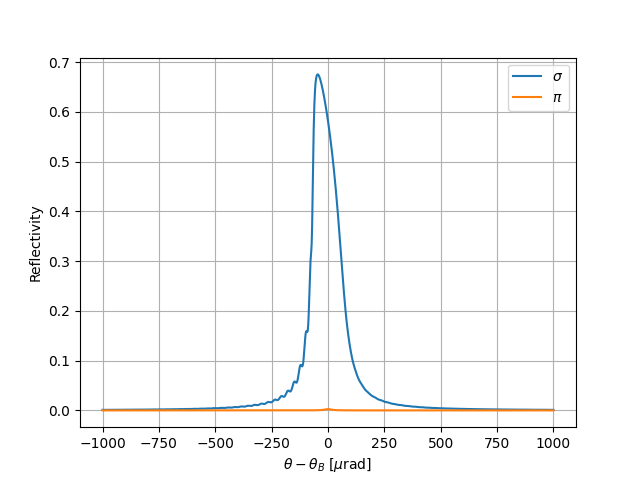
\includegraphics[width=0.85\textwidth]{figures/crystalpyR.png}
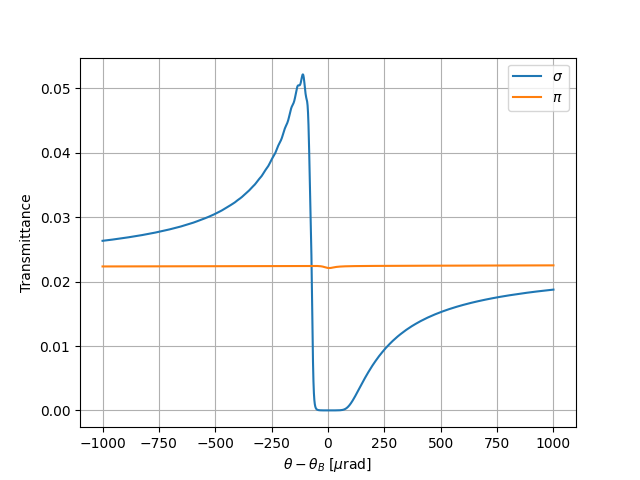
\includegraphics[width=0.85\textwidth]{figures/crystalpyT.png}
\caption{Si 111 perfect crystal plate of thickness \SI{10}{\micro\meter} in Bragg geometry, at 2838~eV, for the $\sigma$ and $\pi$ polarizations, versus the angle $\theta$ from the Bragg angle $\theta_B$ corrected for refraction. a) Reflectivity (reflected beam). b) Transmittance (transmitted or forward-diffracted beam).}
\label{fig:crystalpy}
\end{figure}

The normalized Stokes parameters $P_1=S_1/S_0$ (horizontal/vertical linear polarization) and $P_2=S_2/S_0$ (linear polarization at $\pm45^\circ$) of the transmitted beam were measured with the polarization analyzer of the beamline \cite{Strempfer2013} as a function of the angle of the crystal plate around the Bragg position (48 measurements between $-302$ and $+306$~arcsec). The circular polarization was obtained as $P_3=+\sqrt{1-P_1^2-P_2^2}$, assuming a fully polarized beam (degree of polarization DOP$=1$). Therefore, its sign (the handedness) is not measured, and its modulus is an upper bound of the circular polarization of a partially polarized beam.


% -----------------------------------------------------------------
% -----------------------------------------------------------------
\section{Simulation with SHADOW4}
\label{sec:simulation}
% -----------------------------------------------------------------
% -----------------------------------------------------------------

The phase plate is simulated with the SHADOW4 optical element {\tt S4PlanePhasePlateCrystal} \cite{SanchezdelRio2026efields}. For each ray, the transmission amplitudes $t_\sigma$ and $t_\pi$ are calculated with {\it crystalpy} \cite{Guigay2024} using the direction and photon energy of the ray, and the Jones matrix $\mathrm{diag}(t_\sigma,t_\pi)$ is applied to the electric field of the ray, with the $\sigma$ and $\pi$ directions defined by the diffraction plane. The direction of the ray is not changed. The crystal is aligned at the Bragg angle (corrected for refraction) for 2838~eV, and the rocking scan is simulated by adding a detuning angle $\Delta\theta$ to the crystal angle. The crystal data are from the DABAX library, with the $f_1$, $f_2$ tabulation of Windt, as in the {\it crystalpy} calculations made for the analysis of the measurements.

The plate is rotated around the beam with the azimuthal angle $\alpha$ of the SHADOW4 element. In SHADOW4, a positive detuning $\Delta\theta>0$ increases the glancing angle of the beam on the plate (the incident glancing angle is $\theta_B+\Delta\theta$), so that $\Delta\theta<0$ corresponds to the low-angle side of the reflection. The sense of the measured angle and of the plate rotation are not known in the SHADOW4 frame. We have therefore simulated the four combinations of $\alpha=\pm45^\circ$ and $\Delta\theta=\pm$(measured angle) for a pencil beam (Table~\ref{tab:combinations}). The two signs are determined independently by the measurements:
\begin{itemize}
\item The sign of the detuning is determined by $P_1$. $P_1$ does not depend on the sign of $\alpha$, and it is asymmetric with respect to the Bragg angle, with a deep minimum on one side only (at $+11$~arcsec in the measurements). Only $\Delta\theta=-$(measured angle) places it on the correct side; with $\Delta\theta=+$(measured angle) the curve is reversed. Therefore, positive measured angles correspond to the low-angle side of the reflection.
\item The sign of $\alpha$ is determined by $P_2$. Changing $\alpha$ from $+45^\circ$ to $-45^\circ$ (a mirror reflection of the setup) changes the sign of $P_2$ at all angles. With $\Delta\theta=-$(measured angle), $\alpha=+45^\circ$ reproduces the signs of all the measured values of $P_2$, while $\alpha=-45^\circ$ gives the opposite sign everywhere.
\end{itemize}
Only the combination $\alpha=+45^\circ$ and $\Delta\theta=-$(measured angle) reproduces both $P_1$ and $P_2$, and it is used in the following. The determination of $\alpha$ relies on the sign convention of the measured $P_2$: if it were the opposite of the one used here (Sec.~\ref{sec:conclusions}), $\alpha=-45^\circ$ would be obtained, with the same $P_1$ and the opposite signs of $P_2$ and $P_3$ (handedness). \todo{verify the sense of the angle scan, the rotation of the plate and the sign convention of $P_2$ with the experimental setup}

\begin{table}
\caption{Pencil beam: root mean square differences between the simulated and measured $P_1$ and $P_2$ (48 measured points) for the four combinations of the rotation $\alpha$ of the plate and of the sign of the detuning $\Delta\theta$ with respect to the measured angle, fraction of the measured points (with $|P_k|>0.1$) where the simulated $P_k$ has the same sign as the measured one, and minimum of $P_1$ at the measured angles (measured: $-0.38$ at $+11$~arcsec).}
\label{tab:combinations}
\begin{tabular}{cccccccc}
\toprule
$\alpha$ & $\Delta\theta$ & rms $P_1$ & rms $P_2$ & sign $P_1$ & sign $P_2$ & min $P_1$ & at (arcsec) \\
\midrule
$+45^\circ$ & $-$angle & 0.149 & 0.174 & 0.95 & 1.00 & $-0.92$ & $+18$ \\
$+45^\circ$ & $+$angle & 0.257 & 0.697 & 0.80 & 0.19 & $-0.92$ & $-18$ \\
$-45^\circ$ & $-$angle & 0.149 & 0.996 & 0.95 & 0.00 & $-0.92$ & $+18$ \\
$-45^\circ$ & $+$angle & 0.257 & 0.732 & 0.80 & 0.81 & $-0.92$ & $-18$ \\
\bottomrule
\end{tabular}
\end{table}

The Stokes parameters stored by SHADOW4 for each ray refer to its $\sigma$ direction, which, after the phase plate, is the $\sigma$ direction of the diffraction plane. To compare with the measurements, done in the laboratory frame, an empty element rotated by $-\alpha$ is placed after the phase plate, and the electric field of each ray $j$ is projected onto the right-handed laboratory basis $(\hat{x},-\hat{z})$ (with $\hat{x}$ horizontal, $\hat{z}$ vertical and the beam along $\hat{y}$), giving the Jones vector $(E_1^{(j)},E_2^{(j)})^T$. The Stokes parameters of the beam are the averages over the $N$ traced rays (the lost rays do not contribute)
\begin{eqnarray}\label{eq:stokes_sum}
S_0 &=& \frac{1}{N}\sum_j \left(|E_1^{(j)}|^2+|E_2^{(j)}|^2\right), \nonumber \\
S_1 &=& \frac{1}{N}\sum_j \left(|E_1^{(j)}|^2-|E_2^{(j)}|^2\right), \nonumber \\
S_2 &=& \frac{1}{N}\sum_j 2\,\mathrm{Re}\left(E_1^{(j)}E_2^{(j)*}\right), \nonumber \\
S_3 &=& \frac{1}{N}\sum_j 2\,\mathrm{Im}\left(E_1^{(j)*}E_2^{(j)}\right),
\end{eqnarray}
with the conventions of \cite{SanchezdelRio2026efields} [time factor $e^{-i\omega t}$; $S_3>0$ for left-handed and $S_3<0$ for right-handed circular polarization]. The normalized Stokes parameters are $P_k=S_k/S_0$, and the degree of polarization is $\mathrm{DOP}=(P_1^2+P_2^2+P_3^2)^{1/2}$. Every ray is fully polarized, but the beam is partially polarized (DOP$<1$) when its rays have different polarization states. To compare with the measured $P_3$, we also calculate $\sqrt{1-P_1^2-P_2^2}$ from the simulated $P_1$ and $P_2$, as done with the measurements.

The simulations are done with the script \url{shadow4_desy_p09_scan.py}, which is available with this paper.


% -----------------------------------------------------------------
% -----------------------------------------------------------------
\section{Results}
\label{sec:results}
% -----------------------------------------------------------------
% -----------------------------------------------------------------

\subsection{Pencil beam}
\label{sec:pencil}

A pencil beam is a single ray, monochromatic (2838~eV) and with zero divergence, linearly polarized in the horizontal plane. It is equivalent to the calculation of the transmitted plane wave using the transmission amplitudes \cite{PolarizationDraft}, and it is used here as reference. The rocking scan, with a single ray traced for each detuning angle, is shown in Fig.~\ref{fig:pencil}.

Far from the Bragg angle, the plate does not change the polarization ($P_1\simeq1$). Close to it, within the Darwin width, the plate acts as a polarizer, and the transmitted beam is linearly polarized along the $\pi$ direction of the plate ($P_2\simeq1$); the transmission drops to 0.011, about half of its value far from the Bragg angle (0.021 at the ends of the scan). On both sides of the reflection, the phase difference between the $\sigma$ and $\pi$ components produces circular polarization, with opposite handedness on each side: $|P_3|$ reaches 0.93 (right-handed, $P_3<0$) at $+31$~arcsec, and 0.72 (left-handed) at $-37$~arcsec (the handedness is predicted, not measured, see Sec.~\ref{sec:conclusions}). The largest circular polarization is obtained on the low-angle side of the reflection (positive measured angles), where the transmission is enhanced (up to 0.037).

The simulation reproduces the measured features, their positions, and the signs of $P_1$ and $P_2$. However, the calculated curves have sharper features than the measured ones, like the minimum $P_1=-0.96$ at $+17$~arcsec (the measured minimum is $P_1=-0.38$ at $+11$~arcsec). The root mean square (rms) differences with the 48 measured points are 0.15 for $P_1$ and 0.17 for $P_2$ (Table~\ref{tab:rms}).

\begin{figure}
\centering
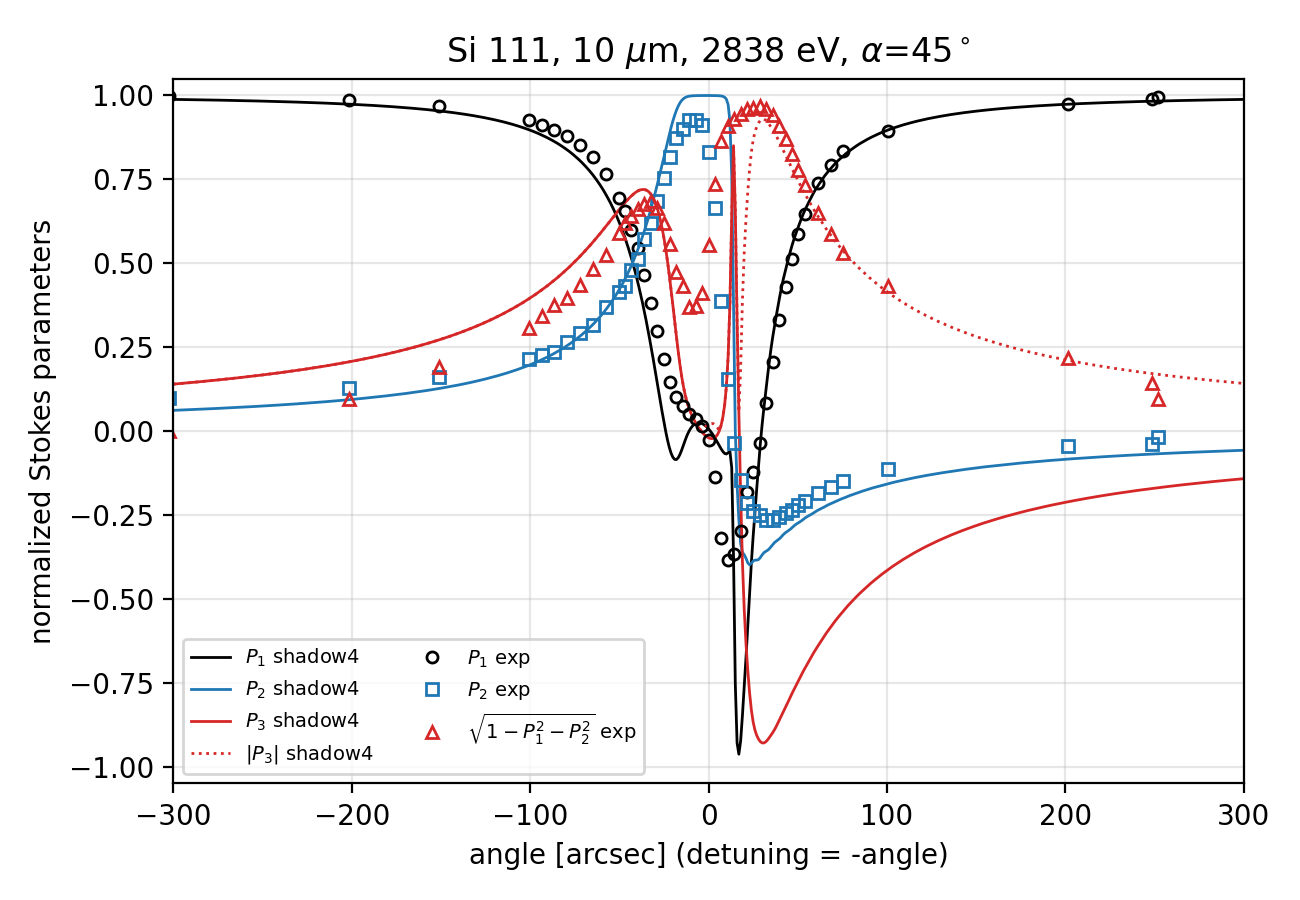
\includegraphics[width=0.95\linewidth]{figures/desy_p09_scan_pencil_beam.png}
\caption{Normalized Stokes parameters of the beam transmitted by a Si 111 phase plate (thickness \SI{10}{\micro\meter}, 2838~eV, $\alpha=45^\circ$) for a horizontally polarized pencil beam, versus the crystal angle. Lines: SHADOW4 (in the laboratory frame); symbols: measurements at the P09 beamline of PETRA III. The measured $P_3$ is $+\sqrt{1-P_1^2-P_2^2}$, and must be compared with $|P_3|$ (dotted line).}
\label{fig:pencil}
\end{figure}


\subsection{Monochromatic undulator beam}
\label{sec:undulator_mono}

The beam of the U32 undulator of P09 is simulated with the SHADOW4 undulator source, monochromatic at 2838~eV (first harmonic, deflection parameter $K=2.382$), with 5000 rays. The electron beam has the rms sizes and divergences of the high-$\beta$ section of PETRA III ($\sigma_x=\SI{141.5}{\micro\meter}$, $\sigma_y=\SI{4.9}{\micro\meter}$, $\sigma'_x=\SI{7.1}{\micro\radian}$, $\sigma'_y=\SI{2.1}{\micro\radian}$). The rms divergences of the photon beam (convolution of the electron beam divergence and the natural divergence of the undulator radiation) are $11.2\times\SI{8.7}{\micro\radian}$ (H$\times$V). The rays are linearly polarized in the horizontal plane ($P_1=0.9999$).

The results are shown in Fig.~\ref{fig:undulator_mono}. They are very similar to those of the pencil beam (Table~\ref{tab:rms}), because the angular spread of the beam (about 2~arcsec rms in the diffraction plane of the plate) is much smaller than the Darwin width (half width 13.3~arcsec). The sharp features are slightly smoothed (the minimum of $P_1$ is $-0.84$), and the beam is slightly depolarized close to the Bragg angle (the minimum DOP is 0.78, at $+15$~arcsec), where $t_\sigma$ and $t_\pi$ change rapidly with the angle.

\begin{figure}
\centering
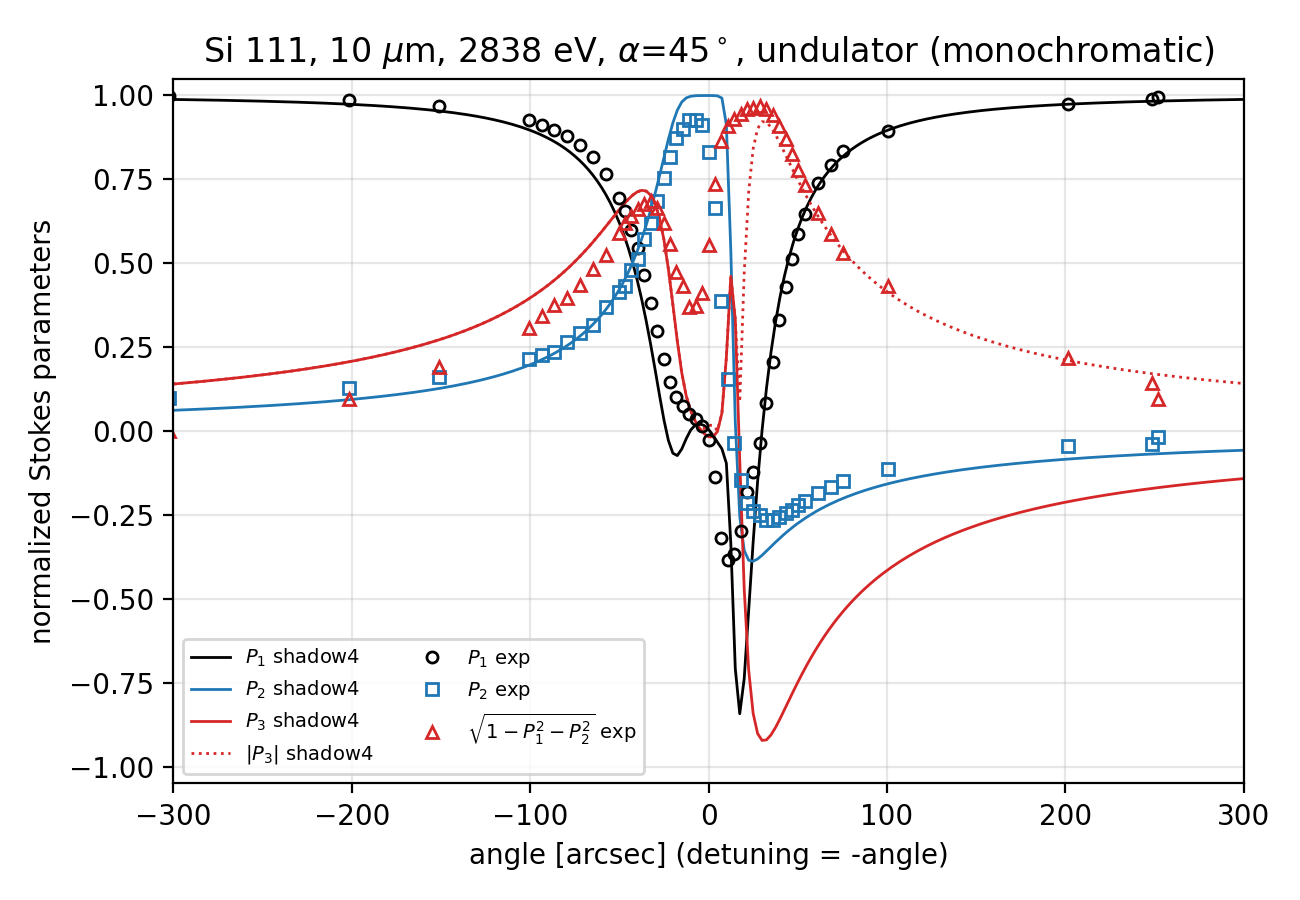
\includegraphics[width=0.95\linewidth]{figures/desy_p09_scan_undulator.png}
\caption{As Fig.~\ref{fig:pencil}, for the monochromatic beam of the P09 undulator (2838~eV, 5000 rays).}
\label{fig:undulator_mono}
\end{figure}


\subsection{Polychromatic undulator beam and Si 111 monochromator}
\label{sec:undulator_poly}

The beam incident on the phase plate is monochromatized by the Si 111 double-crystal monochromator of the beamline. The undulator source is now calculated in the energy interval 2837--2839~eV, and the beam is reflected by two Si 111 crystals (thick crystals, in the non-dispersive $(+,-)$ configuration, deflecting in the vertical plane), aligned for 2838~eV. The crystals of the monochromator are calculated with xraylib. As they deflect in the vertical plane, their $\sigma$ direction is horizontal and the polarization of the beam is practically not changed (as $\theta_B\simeq45^\circ$, their $\pi$ reflectivity is almost zero, and the small vertical component of the beam is removed). The energy distribution of the beam after the monochromator has a width of 0.28~eV FWHM ($\Delta E/E=1.0\times10^{-4}$). At the phase plate, the energy spread is equivalent to an angular spread $\Delta\theta=(\Delta E/E)\tan\theta_B=\SI{97}{\micro\radian}$, or 20~arcsec FWHM, which is comparable to the Darwin width (full width \SI{129}{\micro\radian}, or 26.6~arcsec). This is in agreement with the estimation for P09 of an angular spread larger than 10~arcsec due to the energy spread at energies below 9~keV \cite{Strempfer2013}. The mean energy of the beam after the monochromator is 2837.96~eV, slightly lower than the energy used to align the phase plate (2838~eV); this offset of 0.04~eV shifts the curves by about 3~arcsec, which is negligible here.

The results are shown in Fig.~\ref{fig:undulator_poly}. The energy bandwidth smooths the curves considerably, and the agreement with the measurements of $P_1$ and $P_2$ improves (rms differences 0.094 and 0.070, Table~\ref{tab:rms}): the minimum of $P_1$ is now $-0.50$ at $+10$~arcsec, and the maximum of $P_2$ is 0.96 at $-10$~arcsec. Some differences remain: the simulated minimum of $P_1$ is deeper than the measured one ($-0.38$), the simulated $P_1$ decreases about 10~arcsec earlier than the measured one on the side of negative angles (between about $-60$ and $-30$~arcsec), and the simulated $P_2$ close to $+30$~arcsec is $-0.33$, while the measured one is $-0.27$ (see Sec.~\ref{sec:conclusions} for the possible causes). The beam is now partially polarized close to the Bragg angle (the minimum DOP is 0.52, at $+7.5$~arcsec). The maximum circular polarization is $|P_3|=0.83$ (right-handed, at $+35$~arcsec, with DOP$=0.93$ and a transmission of the plate of 0.033), and 0.68 (left-handed, at $-42.5$~arcsec) on the other side of the reflection.

The measured values of $\sqrt{1-P_1^2-P_2^2}$ (up to 0.97) are larger than the calculated $|P_3|$. This is not a disagreement: for a partially polarized beam, $\sqrt{1-P_1^2-P_2^2}$ includes the unpolarized part of the beam and overestimates $|P_3|$. When the same quantity is calculated from the simulated $P_1$ and $P_2$ (dashed line in Fig.~\ref{fig:undulator_poly}), it reproduces the measurements, including the minimum close to the Bragg angle (rms difference 0.068). This shows that the circular polarization of the beam cannot be obtained from the measured linear polarization alone when the beam is partially polarized, as is the case close to the Bragg angle.

\begin{figure}
\centering
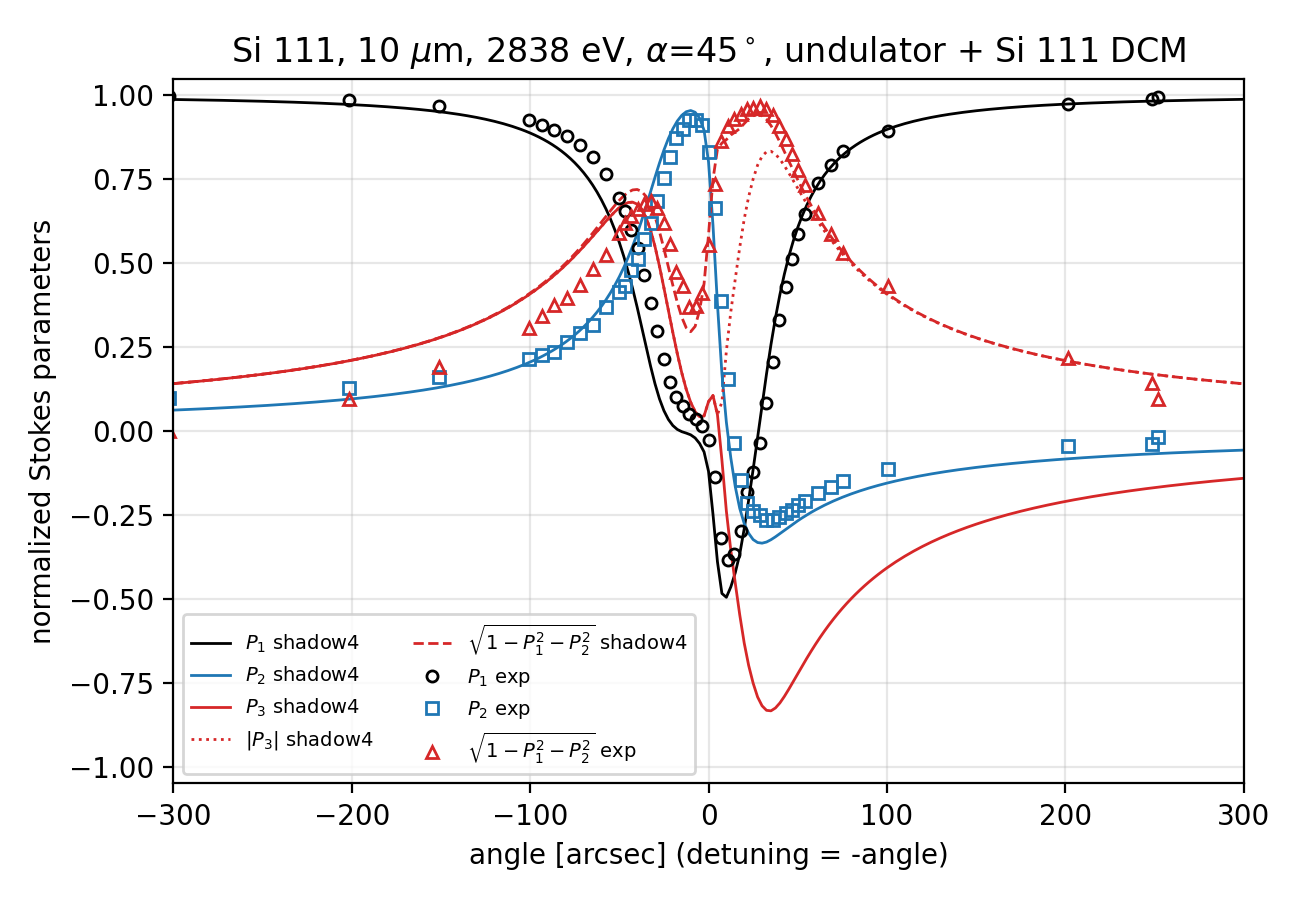
\includegraphics[width=0.95\linewidth]{figures/desy_p09_scan_undulator_polychromatic.png}
\caption{As Fig.~\ref{fig:pencil}, for the beam of the P09 undulator after the Si 111 double-crystal monochromator (5000 rays). The dashed line is $\sqrt{1-P_1^2-P_2^2}$ calculated with the simulated $P_1$ and $P_2$, to be compared with the measured values (triangles).}
\label{fig:undulator_poly}
\end{figure}

\begin{table}
\caption{Root mean square differences between the simulated and measured Stokes parameters (48 measured points), and maximum circular polarization of the simulations. DCM: Si 111 double-crystal monochromator.}
\label{tab:rms}
\begin{tabular}{lcccc}
\toprule
Incident beam & $P_1$ & $P_2$ & $\sqrt{1-P_1^2-P_2^2}$ & $|P_3|_{max}$ \\
\midrule
Pencil beam        & 0.149 & 0.174 & 0.263 & 0.93 \\
Undulator (mono.)  & 0.141 & 0.157 & 0.226 & 0.92 \\
Undulator + DCM    & 0.094 & 0.070 & 0.068 & 0.83 \\
\bottomrule
\end{tabular}
\end{table}


% -----------------------------------------------------------------
% -----------------------------------------------------------------
\section{Discussion and conclusions}
\label{sec:conclusions}
% -----------------------------------------------------------------
% -----------------------------------------------------------------

The SHADOW4 phase plate element, with the polarization of the rays transported by the Jones calculus, reproduces the polarization of the beam transmitted by a Si 111 phase plate measured at the P09 beamline of PETRA III. A calculation with a plane monochromatic wave (or a pencil beam) reproduces the position of the features of the rocking scan and the signs of $P_1$ and $P_2$, but not their amplitudes. The angular distribution of the undulator beam has little effect, because it is much smaller than the Darwin width of the reflection. The energy bandwidth of the Si 111 monochromator, which corresponds to an angular spread at the phase plate comparable to the Darwin width, is the main cause of the smoothing of the measured curves, and must be included to reproduce the measurements.

The simulations give access to quantities that are not measured. The handedness of the circular polarization is predicted, provided that the sign convention of the measured $P_2$ coincides with the one used here (see below); with these conventions, the beam is right-handed on the side of positive measured angles (where the circular polarization is largest) and left-handed on the other side. The degree of polarization of the transmitted beam is also obtained, showing that the beam is partially polarized close to the Bragg angle. In this case, the circular polarization obtained from the measured linear polarization assuming a fully polarized beam is overestimated, and the simulated $|P_3|$ is lower than the measured $\sqrt{1-P_1^2-P_2^2}$.

The remaining differences may be due to the parameters of the simulation (in particular the actual bandwidth and alignment of the monochromator, and the electron beam parameters of the canted 2~m undulator section), to the crystal quality and thickness of the phase plate, and to the uncertainty of the sense of rotation of the plate and of the angle scan, which were deduced here from the measurements. \todo{discuss with the experimentalists}

\paragraph{Open points of this draft.} \todo{to be checked before submission, and removed}
\begin{itemize}
\item {\it Sign conventions of the measurement.} The sense of the measured angle and of the rotation of the plate are not known in the SHADOW4 frame. They were deduced by requiring the simulated signs of $P_1$ and $P_2$ to agree with the measured ones: among $\alpha=\pm45^\circ$ and the two senses of the angle axis, only $\alpha=+45^\circ$ with a detuning equal to minus the measured angle does it (Table~\ref{tab:combinations}). This must be confirmed with the geometry of the experiment.
\item {\it Sign of $P_2$ and handedness.} In the simulation, $P_2=+1$ corresponds to an electric field along $\hat{x}-\hat{z}$, because the laboratory basis $(\hat{x},-\hat{z})$ is right-handed with the beam along $\hat{y}$ (with $\hat{z}$ pointing up). A mirror reflection of the whole setup (left--right) changes the signs of both $P_2$ and $P_3$, but not of $P_1$. Therefore, the predicted handedness follows from the sign of the measured $P_2$, and it is reversed if the convention used at P09 for the $+45^\circ$ direction is the opposite one. The handedness itself is not measured, because $P_3$ is obtained as $+\sqrt{1-P_1^2-P_2^2}$.
\item {\it Measured $P_3$.} It assumes a fully polarized beam (DOP$=1$), and its modulus is an upper bound for a partially polarized beam. It must be compared with the same quantity calculated from the simulated $P_1$ and $P_2$, not with the simulated $|P_3|$.
\item {\it Electron beam.} The electron beam parameters are the PETRA III design values for a 5~m undulator in a high-$\beta$ section ($\varepsilon_x\simeq1$~nm\,rad, $\varepsilon_y\simeq10$~pm\,rad). The undulators of P09 are 2~m long and canted, the design $\beta_x$ for the 2~m undulators is somewhat smaller (16~m instead of 20~m), and the actual emittance of PETRA III is in the range 1.0--1.3~nm\,rad. These differences have little effect here, because the angular spread of the beam is much smaller than the Darwin width.
\item {\it Energy bandwidth.} The bandwidth is calculated with an ideal Si 111 double-crystal monochromator (thick, unstrained crystals, perfectly aligned, without heat load), calculated with xraylib, while the phase plate is calculated with DABAX (Windt $f_1$, $f_2$). The actual bandwidth of the monochromator of P09 at 2838~eV should be confirmed, because it is the main parameter of the comparison. The electron energy spread (0.1\%) is not applied to the undulator emission; it does not change the bandwidth selected by the monochromator.
\item {\it Alignment.} The phase plate is aligned at the Bragg angle (corrected for refraction) for 2838~eV, while the mean energy of the beam after the monochromator is 2837.96~eV (shift of about 3~arcsec). The zero of the measured angle scale is assumed to coincide with this Bragg angle; no shift or scale factor has been fitted.
\item {\it Phase plate.} The plate is assumed to be a perfect, unstrained Si 111 crystal of exactly \SI{10}{\micro\meter}, in symmetric Bragg geometry. Strain, thickness variations or a miscut would broaden or shift the features.
\item {\it Polarization analyzer.} The measured $P_1$ and $P_2$ are taken as exact; the finite extinction of the analyzer and other instrumental effects are not considered.
\item {\it Phase plates at P09.} The description of the phase plates of P09 (diamond for 3.2--14~keV, \SI{10}{\micro\meter} Si for 2.7--3.2~keV) is taken from \cite{Strempfer2013}, where some of them are described as planned; the present equipment should be confirmed.
\end{itemize}


% -----------------------------------------------------------------
\ack{Acknowledgements}
% -----------------------------------------------------------------
\todo{add acknowledgements}

\referencelist{iucr}

\end{document}                    % DO NOT DELETE THIS LINE
